\documentclass[conference]{IEEEtran}
\usepackage{graphicx}
\usepackage{booktabs}
\usepackage{amsmath}
\usepackage{array}
\usepackage{url}
\newcolumntype{L}[1]{>{\raggedright\arraybackslash}p{#1}}

\begin{document}

\title{StepWise: Validation Testing, Result Analysis\\and Discussion (Review-3)}

\author{\IEEEauthorblockN{Siddhi J Salunkhe}
\IEEEauthorblockA{23BDS0243}
\and
\IEEEauthorblockN{Sanvi Saket}
\IEEEauthorblockA{23BDS0210}}

\maketitle

\begin{abstract}
StepWise is an explainable, CPU-only tutor that reads handwritten arithmetic and linear-equation working, verifies each step symbolically, names the misconception and adapts practice. This paper reports its validation testing, result analysis and discussion, revised to answer the Review-3 comments. On held-out data every learned module beats its baseline: the HOG + SVM recognizer reads 92.6\% of symbols by unseen CROHME writers, and a PFA + IRT + recency model predicts real ASSISTments students' next answers with AUC 0.815. New studies then test the system where the review found it weakest. Whole lines are read exactly only 56.7\% of the time; syntax-constrained decoding raises this to 61.4\%, but on full solutions written in real test-writer handwriting, misreads cut diagnosis accuracy from 99.3\% to 35.0\%. A confirm-before-diagnose step restores 93.8\% at the cost of checking about 7 of 14 symbols per page. On 2,120 real erroneous steps by 95 Algebra I students, the mistake classifier detects 94\% of the errors but names the category correctly for only 46\% (majority baseline 53\%); features for in-place simplification, found by error analysis, raise macro-F1 from 0.28 to 0.46 on held-out problems, and adding about 160 labelled real errors to training lifts accuracy to 77\%. Simulated phone capture and two writer populations locate further failure modes, and the simulated adaptive-practice advantage ($d=0.37$) vanishes when learners forget and differ ($d=0.04$). We give the ASSISTments-to-StepWise skill mapping and protocols, with sample sizes, for the photographed-work and classroom studies still to be run.
\end{abstract}

\begin{IEEEkeywords}
handwritten mathematics recognition, support vector machine, knowledge tracing, item response theory, mistake diagnosis, intelligent tutoring systems, validation testing
\end{IEEEkeywords}

\section{Introduction}
Reviews 1 and 2 covered the problem statement, literature survey, architecture and implementation. Review-3 covers validation testing, result analysis and discussion: how each module was tested and what the numbers mean.

The system takes a photo, camera capture or on-screen drawing of handwritten working. It runs an 11-stage pipeline: OpenCV clean-up and segmentation, a symbol recognizer (M1), SymPy step verification \cite{sympy}, a mistake classifier (M2), knowledge tracing with an IRT recommender (M3) and class grouping (M4). Student corrections to misread symbols feed an active-learning loop. All learned parts are classical machine learning (scikit-learn \cite{sklearn}, NumPy, SciPy), run offline on a laptop CPU and total about 6\,MB.

The paper answers four validation questions:
\begin{enumerate}
\item Does the symbol recognizer read real handwriting from writers it has never seen?
\item Does knowledge tracing predict real students' next answers better than simple baselines?
\item Does the learned mistake classifier diagnose misconceptions better than the earlier rule-based system?
\item Do the adaptive practice policy and the class grouping do what they claim on controlled data?
\end{enumerate}

\textit{Revision.} The Review-3 panel raised five concerns. Table~\ref{tab:response} lists them with the change made and where it is reported. Three need data that only a classroom can give (real handwritten student work, real phone photos, a classroom trial). For those we report the closest evidence available now and give a ready-to-run protocol (Section~V-E).

\begin{table}[!t]
\caption{Review-3 Comments and Responses}
\label{tab:response}
\centering
\footnotesize
\setlength{\tabcolsep}{3pt}
\begin{tabular}{L{2.2cm}L{4.25cm}L{1.3cm}}
\toprule
Comment & Response & Where\\
\midrule
C1: 56.7\% exact lines may limit diagnosis & Error sources measured; syntax-constrained decoding (61.4\%); misread-to-diagnosis study; confirm-before-diagnose step & IV-B, IV-C\\
C2: M2 needs real student work & 2,120 real erroneous steps (CogTutorBugs); held-out evaluation; M2 v2; photographed-work protocol & IV-E, V-E\\
C3: phone photos, diverse handwriting & 12 simulated capture conditions; photo-robust binarization; MNIST writer populations; photo protocol & IV-D, V-E\\
C4: ASSISTments-to-StepWise skill mapping & Mapping table with match quality, data volume and per-skill AUC & IV-F\\
C5: classroom validation of practice & Five learner simulators; randomized-trial protocol with sample size & IV-G, V-E\\
\bottomrule
\end{tabular}
\end{table}

Section~II describes the validation protocol and test suite. Section~III gives the setup. Section~IV reports and analyses results. Section~V discusses them and Section~VI concludes.

\section{Validation Testing}
Validation has two layers: model validation on held-out data with no leakage, and functional validation by an automated test suite.

\subsection{Model Validation Protocol}
Each module uses a split that matches how it will meet new data in use. Model and hyperparameter choices are made only on validation data; test sets are touched once (Table~\ref{tab:protocol}). The studies added for the revision (lower block) evaluate the deployed models; their test data is never used for training or for choices.

\begin{table*}[!t]
\caption{Validation Protocol per Module}
\label{tab:protocol}
\centering
\footnotesize
\begin{tabular}{L{2.6cm}L{4.0cm}L{3.5cm}L{3.6cm}L{2.2cm}}
\toprule
Module / study & Training data & Validation (for choices) & Test (reported) & Split rule\\
\midrule
M1 Symbol recognizer & CROHME train (6,271 symbols) \cite{crohme}, HASYv2 (3,335 symbols, 144 writers) \cite{hasy}, 12,210 font glyphs & 15\% held-out CROHME-train expressions + 25\% held-out fonts; mean macro-F1 & Official CROHME 2014/16/19 test: 1,821 symbols, 127 expressions & Writer-disjoint; font-disjoint\\
M2 Mistake classifier & 3,150 synthetic solutions & 5-fold stratified CV on the 80\% & 630 synthetic solutions (70 per class) & Stratified 80/20\\
M3 Knowledge tracing (real) & ASSISTments 2009 \cite{assist}, 80\% of 4,151 students & Validation students from training split (Rasch L2) & 74,867 next-answer predictions & Learner-disjoint 80/20\\
M3 Knowledge tracing (sim.) & 600 simulated learners, 93,671 attempts & -- & Held-out learners & Learner-disjoint 80/20\\
M3 Recommender policy & Simulated learners & -- & 40 items per learner, 5 seeds & Repeated simulation\\
M4 Class grouping & 120 simulated students, 4 planted archetypes & $k$ by silhouette (2--6) & ARI vs planted groups & Unsupervised\\
\midrule
Misreads $\rightarrow$ diagnosis (C1) & Deployed M1 + M2 & Gate threshold $\tau$ on 210 validation pages & 420 solutions (unseen seed) written with CROHME test-writer glyphs & Writer-disjoint\\
Phone capture (C3) & Deployed M1 + M2 & -- & The 420 pages under 12 simulated capture conditions & Same pages\\
Writer populations (C3) & Deployed M1 & -- & MNIST test: 5,001 digits by students, 4,999 by Census staff \cite{mnist,qmnist} & Dataset-disjoint\\
M2 on real errors (C2) & Synthetic only (no real data) & Error analysis on 30\% of problem templates & 1,552 real errors from the other 70\% (CogTutorBugs \cite{cogtutorbugs}) & Template-disjoint\\
Policy robustness (C5) & Deployed learner model & -- & 5 simulators $\times$ 3 policies, 150 learners $\times$ 5 seeds & Repeated simulation\\
\bottomrule
\end{tabular}
\end{table*}

Three safeguards prevent optimistic results. First, CROHME test writers never appear in training. Second, the fonts-only model is kept as a control to show the effect of real data. Third, every learned model is compared with at least one non-learned or simpler baseline (rules, EMA recency, random policy, majority class).

\subsection{Label Validation}
CROHME labels whole expressions, not symbols, so symbol labels come from count alignment: the app's segmenter runs on each linear expression, and crops are labelled left to right only when the symbol count equals the LaTeX token count. A manual check of 80 random crops found 79 correct (98.75\%). For CogTutorBugs, SymPy decides which student steps are mathematically wrong (the new equation has a different solution set); their tutor labels are then mapped to StepWise categories by a fixed, published table (Section~IV-E).

\subsection{Functional Validation (Test Suite)}
The backend has 171 automated pytest cases (counted after parametrization) across 14 test modules (Table~\ref{tab:tests}). The Review-3 version of this table listed per-module counts that did not add up to its total; the counts below are taken from the test collector. The cases cover four types: unit tests of each feature and metric, model tests that check a learner recovers known parameters, integration tests of the full pipeline, and API tests of each user flow. The frontend is validated by a successful production build.

\begin{table}[!t]
\caption{Automated Test Suite}
\label{tab:tests}
\centering
\footnotesize
\begin{tabular}{L{2.9cm}cL{3.7cm}}
\toprule
Module & Tests & Validates\\
\midrule
ml & 28 & Symbol and mistake features; mini training run\\
validation & 27 & Decoder, photo binarization, crash fixes, gate, study helpers\\
learning\_models & 23 & BKT/Rasch recovery, recommender, clustering\\
api\_endpoints & 13 & Submission, progress, quiz endpoints\\
math\_parser & 13 & SymPy parsing without \texttt{eval}\\
ml\_api & 12 & ML Lab, correction, confirmation, retraining\\
benchmark\_metrics & 11 & CER, WER, exact match, macro-F1\\
quiz\_service & 11 & Item bank answers verified with SymPy\\
providers & 8 & ML, demo and optional OCR providers\\
diagnosis & 7 & Step-error localisation, guardrails\\
upload\_validation & 7 & File type, size, corrupt images\\
database\_operations & 5 & Persistence of students, mastery\\
benchmark\_service & 3 & Benchmark summary over a manifest\\
preprocessing & 3 & OpenCV clean-up stages\\
\bottomrule
\end{tabular}
\end{table}

\section{Experimental Setup}
All experiments run on a laptop CPU with a fixed random seed (0). The full training run takes about 8 minutes with real data, and the validation studies (\texttt{python -m app.ml.validate}) about 30 minutes.

\subsection{Environment}
Python 3.10+, scikit-learn 1.5.2, NumPy 1.26.4, SymPy 1.13.2, OpenCV 4.10, FastAPI 0.115 and SQLAlchemy 2.0 on the backend; React with Vite on the frontend. No GPU, neural network or API key is used. Every number in Section~IV is regenerated by the training or validation scripts and stored as JSON reports.

\subsection{Models and Hyperparameters}
\begin{itemize}
\item \textbf{M1} (374 features: HOG \cite{hog} 324 + 7$\times$7 zoning 49 + log aspect 1): SVM \cite{svm} (RBF, $C=10$, $\gamma$ = scale); Random Forest (200 trees); Logistic Regression ($C=0.5$); kNN ($k=5$, distance-weighted). Added in the revision: syntax-constrained decoding and photo-robust page binarization (Section~IV-B, IV-D).
\item \textbf{M2} (42 named features, v2): Random Forest \cite{rf} (300 trees, min leaf 2); HistGradientBoosting (200 iterations, lr 0.1); Decision Tree (depth 8); Logistic Regression ($C=1$); rule-based baseline.
\item \textbf{M3}: EMA, BKT \cite{bkt} (EM per skill), PFA \cite{pfa}, PFA + Rasch IRT \cite{rasch}, PFA + IRT + recency; Rasch L2 chosen from \{0.05, 1.0, 5.0\} $\rightarrow$ 1.0.
\item \textbf{M4}: K-Means ($k$ from 2--6 by silhouette, $n_{init}=10$) vs agglomerative (Ward).
\end{itemize}

\subsection{Evaluation Metrics}
Classification (M1, M2) uses accuracy, macro-F1 and confusion matrices; expression reading uses exact-match rate and character error rate (CER; Levenshtein distance / reference length); next-answer prediction (M3) uses ROC AUC, RMSE and log-loss; the policy uses the share of skills mastered after 40 items and an expected post-test score; clustering uses adjusted Rand index (ARI) \cite{ari}, silhouette and Davies--Bouldin. Accuracies on real data carry bootstrap 95\% confidence intervals (2,000 resamples). Macro-F1 is the main classification metric because small classes such as `/' (9 test symbols) would be hidden by plain accuracy:
\begin{equation}
\text{Macro-F1} = \frac{1}{K}\sum_{k=1}^{K} \frac{2 P_k R_k}{P_k + R_k}.
\end{equation}

\section{Results and Result Analysis}
Every learned module beats its baseline on held-out data; the largest single gain is real training data, which lifts symbol accuracy on unseen writers from 55.3\% to 92.6\% (Table~\ref{tab:headline}). Sections~IV-B to IV-G then test the system end to end and on real student data, where the picture is less favourable.

\begin{table*}[!t]
\caption{Headline Results (Seed 0)}
\label{tab:headline}
\centering
\footnotesize
\begin{tabular}{L{2.8cm}L{3.4cm}L{2.8cm}L{3.2cm}L{3.2cm}}
\toprule
Module & Data & Selected model & Test result & Best baseline\\
\midrule
M1 Symbol recognizer & Real (CROHME test, unseen writers) & SVM (RBF) & 92.6\% acc., macro-F1 0.899 & Fonts-only training: 55.3\%\\
M3 Knowledge tracing & Real (ASSISTments 2009) & PFA + IRT + recency & AUC 0.815 & EMA: 0.811\\
M2 Mistake classifier & Synthetic & Random Forest & Macro-F1 0.992 & Rule-based: 0.311\\
M2 on real errors & Real (CogTutorBugs, held out) & Random Forest v2 & 52.1\% category acc., macro-F1 0.460 & Majority class: 53.2\%, macro-F1 0.174\\
M3 Practice policy & Simulated & Adaptive (BKT + IRT) & 74.1\% skills mastered; vanishes with forgetting (Table~\ref{tab:robust}) & Random: 63.8\%\\
M4 Class grouping & Simulated & K-Means ($k=5$) & ARI 0.82 & Agglomerative agrees at ARI 0.86\\
\bottomrule
\end{tabular}
\end{table*}

\subsection{M1: Symbol Recognition on Real Handwriting}
Table~\ref{tab:data} shows the same SVM trained on three datasets. The fonts-only model scores 0.975 macro-F1 on held-out fonts but 0.573 on real writers, so printed fonts are a poor stand-in for handwriting. Real-only and fonts + real are tied on handwriting; fonts + real was chosen on validation (0.930 vs 0.899) because it also reads printed worksheets, where real-only misreads some printed `4's.

\begin{table}[!t]
\caption{Effect of Training Data (SVM, CROHME Test)}
\label{tab:data}
\centering
\footnotesize
\begin{tabular}{lcccc}
\toprule
Training data & Acc. & Macro-F1 & Expr. exact & CER\\
\midrule
Fonts only & 0.553 & 0.573 & 0.220 & 0.452\\
Real only & 0.927 & 0.913 & 0.575 & 0.120\\
\textbf{Fonts + real} & \textbf{0.926} & 0.899 & \textbf{0.575} & \textbf{0.110}\\
\bottomrule
\end{tabular}
\end{table}

\begin{table}[!t]
\caption{Algorithm Comparison (Fonts + Real Training)}
\label{tab:algo}
\centering
\footnotesize
\begin{tabular}{lcccc}
\toprule
Algorithm & Val. score & Test acc. & Test F1 & Fit (s)\\
\midrule
\textbf{SVM (RBF)} & \textbf{0.930} & \textbf{0.926} & \textbf{0.899} & 32.8\\
Logistic Regression & 0.911 & 0.903 & 0.880 & --\\
Random Forest & 0.916 & 0.900 & 0.875 & 6.7\\
kNN & 0.907 & 0.878 & 0.848 & 0.0\\
\bottomrule
\end{tabular}
\end{table}

Validation ranking matches test ranking for the winner (Table~\ref{tab:algo}), which supports the selection protocol. Results are stable across years: 91.1\% (2014, $n=461$), 93.1\% (2016, $n=666$) and 93.1\% (2019, $n=694$). Fig.~\ref{fig:f1} shows that 14 of 17 classes reach F1 $\geq$ 0.89; the slash is the outlier at 0.545, but it has only 9 test samples. The most frequent confusions are `1' read as `/' (12 of 188), `x' as `1' (7), `=' as `$-$' (5) and `9' as `3' (5): all shape-similar pairs.

\begin{figure}[!t]
\centering
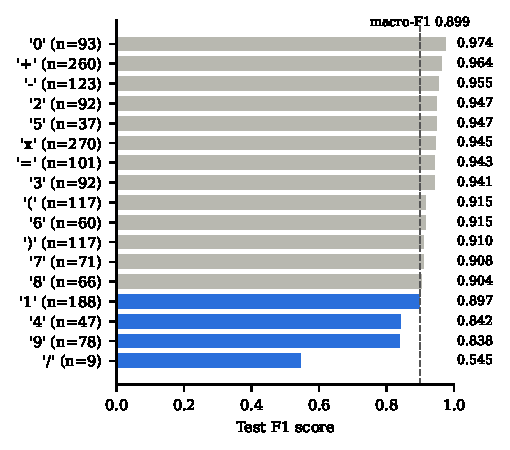
\includegraphics[width=\columnwidth]{fig1.pdf}
\caption{Per-class test F1 of the SVM symbol recognizer on CROHME 2014/16/19. Blue: classes below the macro average (dashed).}
\label{fig:f1}
\end{figure}

\subsection{From Symbols to Lines (C1)}
The deployed recognizer, refit on training plus validation data, reads 72 of the 127 test expressions exactly (56.7\%; the 57.5\% in Table~\ref{tab:data} is the model before refitting). The Review-3 version explained the gap from 92.6\% with ``about 4 symbols per expression''. That figure was wrong: it averaged over all 468 aligned expressions, but exact match is measured on the 127 that use only StepWise's 17 symbols, and these average 9.35 symbols. With the deployed model's 92.4\% symbol accuracy, independent errors predict 54.2\% exact lines, close to the observed 56.7\%. Line length, not a hidden defect, drives the gap (Table~\ref{tab:reading}): short lines of up to 5 symbols, the size of most student steps, are read exactly 86\% of the time.

\begin{table}[!t]
\caption{Whole-Line Reading, 127 CROHME Test Expressions}
\label{tab:reading}
\centering
\footnotesize
\begin{tabular}{lccc}
\toprule
Lines & $n$ & Argmax & Syntax-constrained\\
\midrule
1--5 symbols & 51 & 0.863 & 0.863\\
6--10 symbols & 26 & 0.500 & 0.538\\
$>$10 symbols & 50 & 0.300 & \textbf{0.400}\\
\midrule
All & 127 & 0.567 & \textbf{0.614}\\
Well-formed student lines & 123 & 0.577 & \textbf{0.634}\\
\bottomrule
\end{tabular}
\end{table}

Of the 55 failed lines, 26 are segmentation errors (25 touching symbols merged, 1 split) and 29 are symbol substitutions. Many substitutions produce lines no student writes, such as `1 + ) + / + 1'. \textit{Syntax-constrained decoding} therefore keeps each symbol's top three SVM classes and chooses, by Viterbi search over (symbol kind, bracket depth), the most probable sequence that is a well-formed line: no two operators in a row, balanced brackets, no line ending in an operator. It uses syntax only, never arithmetic, so a student's wrong answer is still read as written. It repairs 7 lines and breaks 1, a CROHME fragment that no student writes (`(2001)4373'), raising exact match to 61.4\% (Table~\ref{tab:reading}). Segmentation errors are untouched and remain the largest error source.

\subsection{From Reading to Diagnosis (C1)}
How much does a misread cost the diagnosis? We generated 420 fresh synthetic solutions (60 for each of the 7 categories that can be written with the 17 symbols; a seed M2 never saw) and wrote each in real handwriting by pasting CROHME 2014/16/19 test-writer glyphs at their natural relative size and height. The pages average 14.3 symbols over 2--3 lines. Each page was read by the deployed M1 and diagnosed by the deployed M2, and compared with diagnosing its true transcription.

\begin{figure}[!t]
\centering
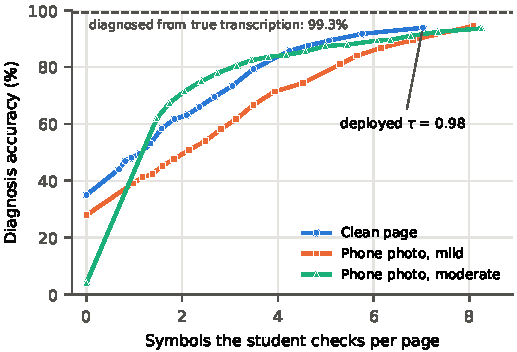
\includegraphics[width=\columnwidth]{fig2.pdf}
\caption{Diagnosis accuracy on 420 solutions written in CROHME test-writer handwriting, against the symbols a student checks per page as the confirm-before-diagnose threshold $\tau$ rises (one marker per $\tau$ from 0.30 to 0.98; $x=0$: no confirmation).}
\label{fig:gate}
\end{figure}

The comment is borne out. Only 16.7\% of clean pages are read exactly, and diagnosis accuracy falls from 99.3\% on the true transcription to 35.0\% (Fig.~\ref{fig:gate}, $x=0$). Worse, 56.7\% of correct solutions are marked wrong because a misread digit looks like an arithmetic slip. A tutor must not do this, so StepWise now has a \textit{confirm-before-diagnose} step: symbols read with confidence below $\tau$ are highlighted, and no diagnosis is given until the student has checked them (one tap per symbol, or ``reading is right''). $\tau$ was chosen on 210 separate validation pages as the smallest value at which at most 5\% of pages are diagnosed differently from their true transcription: $\tau=0.98$. On the test pages this restores 93.8\% accuracy (macro-F1 0.946) and cuts correct work marked wrong to 5.0\%. The cost is real: about 7.0 of the 14.3 symbols are highlighted per page, and 0.25 lines per page must be retyped because of segmentation errors. Fig.~\ref{fig:gate} shows the trade-off; for example, $\tau=0.9$ gives 85.7\% with 4.2 checks per page.

\subsection{Phone Photos and Writer Populations (C3)}
\textit{Simulated capture.} No phone photos of student work exist yet (Section~V-E), so the 420 pages were put through a capture simulator with one factor at a time and three combined severities: off-white textured paper with ballpoint ink, notebook rules and margin, a lighting gradient losing 45\% of brightness, a soft cast shadow, perspective tilt with rotation, defocus blur, sensor noise with JPEG compression, and 60\% resolution. This exposed a design flaw. The recognizer binarized with one global Otsu threshold, which turns a shadow or a lighting gradient into ink and merges ruled lines with the writing. A photo-robust page binarization now divides the image by a background estimate (a grey-level closing much wider than any stroke) and erases ink runs longer than half the page and four symbol heights. On evenly lit images it returns the input unchanged, so all CROHME results are identical. Table~\ref{tab:capture} gives the effect.

\begin{table}[!t]
\caption{Simulated Phone Capture: Reading (CER) and Diagnosis}
\label{tab:capture}
\centering
\footnotesize
\begin{tabular}{lccccc}
\toprule
 & \multicolumn{2}{c}{CER} & \multicolumn{3}{c}{Diagnosis acc.}\\
Condition & Otsu & New & None & Conf. & Checks\\
\midrule
Clean page & 0.13 & 0.13 & 0.350 & 0.938 & 7.0\\
Paper and pen & 0.12 & 0.12 & 0.355 & 0.943 & 7.2\\
Ruled paper & 0.90 & 0.16 & 0.307 & 0.945 & 8.5\\
Uneven lighting & 0.74 & 0.10 & 0.369 & 0.952 & 7.1\\
Cast shadow & 0.80 & 0.12 & 0.379 & 0.964 & 7.3\\
Tilt & 0.15 & 0.15 & 0.326 & 0.952 & 7.9\\
Blur & 0.19 & 0.19 & 0.205 & 0.902 & 8.9\\
Noise + JPEG & 0.13 & 0.13 & 0.379 & 0.933 & 7.0\\
Low resolution & 0.20 & 0.20 & 0.212 & 0.893 & 9.0\\
\midrule
Phone, mild & 0.51 & 0.16 & 0.279 & 0.945 & 8.1\\
Phone, moderate & 0.93 & 0.69 & 0.041 & 0.936 & 8.2\\
Phone, severe & 0.93 & 0.86 & 0.012 & 0.988 & 4.5\\
\bottomrule
\end{tabular}
\end{table}

With the new binarization, paper texture, uneven lighting, shadows and sensor noise leave diagnosis without confirmation at the clean-page level, and rules and tilt cost a few points. Blur and low resolution hurt most among single factors (about 21\%), likely because smeared strokes join neighbouring symbols, which the segmenter cannot split. Combined conditions collapse it (4.1\% at moderate severity). With confirmation, accuracy stays at 89--99\%, but at moderate and severe capture the student retypes about two lines per page, which amounts to typing the work.

\textit{Writer populations.} MNIST test digits \cite{mnist} were never used for training. They were written with pen on paper forms and scanned, unlike CROHME's tablet ink. Following the QMNIST reconstruction \cite{qmnist}, the first 5,001 were written by about 250 US high-school students and the last 4,999 by 48 Census Bureau employees. The recognizer reads 86.3\% of the students' digits and 85.0\% of the employees', against 91.0\% on CROHME test digits. The loss is concentrated in `1', often written slanted and read as `/' (recall 66\% for students and 48\% for employees, against 87\% on CROHME), and in `4' read as `9'. Context helps in a full line, where the constrained decoder rejects a `/' that cannot be an operator, but isolated digits show a real domain gap.

\subsection{M2: Mistake Classification}
\begin{table}[!t]
\caption{Mistake Classifier v2 (630 Held-out Synthetic Solutions)}
\label{tab:mistake}
\centering
\footnotesize
\begin{tabular}{lccc}
\toprule
Algorithm & CV macro-F1 & Test F1 & Fit (s)\\
\midrule
\textbf{Random Forest} & \textbf{0.991 $\pm$ 0.003} & \textbf{0.992} & 0.24\\
Gradient Boosting & 0.991 $\pm$ 0.003 & 0.991 & 9.79\\
Logistic Regression & 0.988 $\pm$ 0.006 & 0.987 & 0.28\\
Decision Tree & 0.948 $\pm$ 0.013 & 0.940 & 0.00\\
Rule-based (previous) & -- & 0.311 & --\\
\bottomrule
\end{tabular}
\end{table}

On synthetic data (Table~\ref{tab:mistake}) the Random Forest makes 5 errors in 630: one manipulation error labelled a sign error, and four confusions among ``couldn't read'', ``not enough to check'' and ``correct''. The rule-based system (accuracy 0.387), by contrast, sends 37 of 70 arithmetic slips and 40 of 70 sign errors to ``final answer mismatch'': it sees that the answer is wrong but cannot say why. Table~\ref{tab:mistake} is the v2 model. The Review-3 model (v1, 33 features) scored 0.994, and v2 was introduced for the reason below.

\textit{Real student errors (C2).} CogTutorBugs \cite{cogtutorbugs} holds 5,339 steps on which 95 Algebra I students using the Cognitive Tutor made an error the tutor caught, each stored as the equation before, the student's equation after and one of 19 error labels. The steps are typed, not handwritten, so this tests diagnosis on its own, which is the part trained only on synthetic data. Of the 5,220 parseable steps, SymPy finds 2,120 mathematically wrong (the new equation has different solutions) and 3,100 valid but unhelpful, such as adding instead of subtracting to remove a term. StepWise gives no strategy feedback, so for the latter the right answer is ``valid''. Wrong steps were mapped to StepWise categories: sign (4 labels, e.g. ``negative times negative''), wrong operation, arithmetic (fraction simplified to a wrong value) and manipulation (e.g. dropping the variable). Each step was diagnosed as two-line working with no answer key.

\begin{table}[!t]
\caption{M2 on Real Student Errors (CogTutorBugs)}
\label{tab:cogtutor}
\centering
\footnotesize
\setlength{\tabcolsep}{3.5pt}
\begin{tabular}{lccc}
\toprule
 & Rules & M2 v1 & M2 v2\\
\midrule
Wrong steps flagged as wrong & 0.108 & 0.941 & 0.957\\
Valid steps accepted & 0.996 & 0.993 & 0.993\\
\midrule
\multicolumn{4}{l}{\textit{Category, 1,552 errors on held-out templates (majority 0.532)}}\\
Accuracy & 0.019 & 0.463 & 0.521\\
\quad 95\% CI & -- & 0.439--0.488 & 0.497--0.546\\
Macro-F1 & 0.028 & 0.279 & 0.460\\
Recall: sign & -- & 0.690 & 0.696\\
Recall: wrong operation & -- & 0.013 & 0.510\\
Recall: arithmetic & -- & 0.026 & 0.051\\
Recall: manipulation & -- & 0.613 & 0.618\\
\bottomrule
\end{tabular}
\end{table}

The answer to the comment is mixed (Table~\ref{tab:cogtutor}). \textit{Detection} transfers: v1 flags 94.1\% of the real wrong steps, accepts 99.3\% of the valid ones, and calls only 1.8\% of the wrong steps correct. The rule-based system flags just 10.8\%, because without an answer key it can only check purely numeric lines. \textit{Naming the category} does not transfer. v1 is right for only 46.3\% of the held-out errors, below the 53.2\% majority class, and its macro-F1 of 0.279 is far from the synthetic 0.994. Wrong-operation and arithmetic errors are almost never recognised. Error analysis on the 30\% development templates showed why. Real students simplify one side of an equation in place ($-75x = 4 - 54$ becomes $-75x = 58$), and the slip is in that small computation. Our features checked such computations only on purely numeric lines, and our generator never produced them. M2 v2 adds nine \texttt{local\_*} features, which apply the existing numeric checks (operator swap, sign flip, off by 1--2) to a part simplified in place, and adds generators for such slips. Trained still only on synthetic data, v2 reaches 52.1\% on the held-out templates. Wrong-operation recall rises from 1\% to 51\% and macro-F1 from 0.279 to 0.460. Accuracy, however, is still not above the majority class (its 95\% CI includes 53.2\%), and arithmetic slips, mostly fractions simplified to a wrong value, are still rarely recognised (5\%). What is missing is labelled real data. In a problem-grouped 5-fold cross-validation, adding real labelled errors to the synthetic training data lifts v2 to 77.2\% accuracy with 10\% of the training folds (about 160 errors) and to 83.3\% with all of them, whereas v1's features reach only 59.2\% with all of them. The v2 features carry the signal, and a modest labelled real set would exploit it. Section~V-E gives the protocol for collecting real handwritten work.

\subsection{M3: Knowledge Tracing and the Skill Mapping (C4)}
\begin{table}[!t]
\caption{Next-Answer Prediction, ASSISTments 2009 (74,867 Predictions)}
\label{tab:kt}
\centering
\footnotesize
\begin{tabular}{lccc}
\toprule
Model & AUC & RMSE & Log-loss\\
\midrule
\textbf{PFA + IRT + recency} & \textbf{0.815} & \textbf{0.396} & \textbf{0.476}\\
EMA (recency baseline) & 0.811 & 0.403 & 0.494\\
PFA & 0.787 & 0.404 & 0.490\\
PFA + Rasch IRT & 0.781 & 0.413 & 0.525\\
BKT (EM, per skill) & 0.771 & 0.408 & 0.513\\
\bottomrule
\end{tabular}
\end{table}

On simulated learners the ranking is reversed: BKT leads (AUC 0.835) ahead of PFA (0.832) and EMA (0.820). BKT recovers the simulator's true parameters with mean absolute error 0.021, and Rasch difficulties correlate 0.75 with true difficulty.

\textit{Skill mapping.} The ASSISTments benchmark (Table~\ref{tab:kt}) uses all 110 ASSISTments skills and needs no mapping. The mapping serves one purpose only: to fit the BKT parameters StepWise deploys for its own eight skills on real students. Each StepWise skill was matched by name and scope to the ASSISTments skills covering the same operation. ASSISTments 2009 publishes no problem text, so no item-level alignment is possible. Table~\ref{tab:skills} gives the matches, how close they are, the data behind each and next-answer AUC restricted to those skills. Four points follow. (i) S1, S3 and S4 match directly. S5 and S6 are close: ``Two or fewer steps'' also contains one-step equations. S2 is partial, since ASSISTments has no whole-number division skill and positive-decimal multiplication and division stand in. S7 is approximate, since multi-step solving applies inverse operations repeatedly but is not specific to moving a term across `='. (ii) S8, equations with negative numbers, has no counterpart and keeps parameters fitted on simulated learners. (iii) The mapped skills hold 20.7\% of all ASSISTments answers. (iv) Several fitted parameters sit on the EM bounds (guess $G=0.3$ for S2, S3 and S5--S7; learn rate $T=0.6$ for S7), a sign that the skill-builder data, which ends after three correct answers in a row, constrains them weakly. The per-skill test AUCs show that the selected PFA + IRT + recency model predicts next answers on the mapped skills almost as well as overall (0.71--0.83 against 0.815). BKT, which StepWise uses for mastery, is weakest exactly where the match is weakest: 0.54 on S7, barely above chance, against 0.77 for the selected model. StepWise's S7 mastery estimate should therefore be treated as weak until it is refitted on StepWise's own practice logs.

\begin{table*}[!t]
\caption{ASSISTments-to-StepWise Skill Mapping. Seq.: Learner--Skill Sequences; Deployed BKT Parameters; Next-Answer AUC of BKT and of the Selected PFA + IRT + Recency Model on Test Learners, Restricted to the Mapped Skills}
\label{tab:skills}
\centering
\footnotesize
\begin{tabular}{L{2.9cm}L{5.0cm}lrrccc}
\toprule
StepWise skill & ASSISTments skill(s) & Match & Seq. & Answers & $L_0$/$T$/$G$/$S$ & BKT & Selected\\
\midrule
S1 Whole-number $+$/$-$ & Addition Whole Numbers; Subtraction Whole Numbers & direct & 1,891 & 12,437 & .89/.03/.09/.21 & 0.772 & 0.789\\
S2 Multiply/divide & Multiplication Whole Numbers; Multiplication and Division Positive Decimals & partial & 393 & 2,080 & .75/.11/.30/.09 & 0.713 & 0.736\\
S3 Integers with negatives & Addition and Subtraction Integers; Multiplication and Division Integers & direct & 2,126 & 36,054 & .78/.02/.30/.14 & 0.761 & 0.831\\
S4 Order of operations & Order of Operations All; Order of Operations +,-,/,* () positive reals & direct & 1,315 & 7,731 & .72/.08/.23/.28 & 0.669 & 0.713\\
S5 One-step equations & Solving for a variable & close & 307 & 1,792 & .66/.06/.30/.16 & 0.686 & 0.738\\
S6 Two-step equations & Equation Solving Two or Fewer Steps & close & 961 & 24,253 & .66/.03/.30/.24 & 0.662 & 0.744\\
S7 Moving terms across `=' & Equation Solving More Than Two Steps & approximate & 412 & 8,115 & .55/.60/.30/.22 & 0.541 & 0.773\\
S8 Equations with negatives & none (simulated parameters) & none & -- & -- & .13/.08/.07/.20 & -- & --\\
\bottomrule
\end{tabular}
\end{table*}

\begin{table}[!t]
\caption{Practice Policy (40 Items per Learner, 5 Seeds)}
\label{tab:policy}
\centering
\footnotesize
\begin{tabular}{lcc}
\toprule
Policy & Skills mastered & Wasted practice\\
\midrule
\textbf{Adaptive} (BKT + IRT) & \textbf{0.741 $\pm$ 0.008} & \textbf{28\%}\\
Round-robin & 0.640 $\pm$ 0.010 & 47\%\\
Random & 0.638 $\pm$ 0.013 & 49\%\\
\bottomrule
\end{tabular}
\end{table}

\subsection{M3: Practice Policy and Its Robustness (C5)}
The adaptive policy picks the least-mastered skill at about 70\% predicted success. In the Review-3 simulation it masters 10.3 percentage points more skills than random and wastes 21 points less practice on already-learned skills (Table~\ref{tab:policy}). That simulator is BKT + IRT-like and so favours a BKT-based policy. To test how much the advantage depends on it, the deployed learner model (BKT for S1--S7 fitted on real students) chose items for learners from five simulators. These were the original; one calibrated with the real-student parameters of Table~\ref{tab:skills}; one where a learned skill is forgotten with probability 0.02 whenever another is practised; one where learning rates vary between learners (log-normal, s.d.\ 0.6); and all of these combined. Besides the latent share of skills learned, we score an expected post-test (16 mid-difficulty items, 2 per skill), which a classroom study can actually observe.

\begin{table}[!t]
\caption{Adaptive vs Random Practice Under Five Simulators}
\label{tab:robust}
\centering
\footnotesize
\begin{tabular}{lcccc}
\toprule
 & \multicolumn{2}{c}{Skills learned} & Post-test & \\
Simulator & Adaptive & Random & gain (pts) & $d$\\
\midrule
Original & 0.702 & 0.638 & +5.0 & 0.37\\
Real-calibrated & 0.864 & 0.779 & +5.1 & 0.50\\
Heterogeneous & 0.711 & 0.649 & +4.7 & 0.29\\
Forgetting & 0.449 & 0.423 & +2.3 & 0.17\\
All combined & 0.487 & 0.481 & +0.5 & 0.04\\
\bottomrule
\end{tabular}
\end{table}

The advantage survives learners calibrated on real students (+8.5 points of skills learned, post-test $d=0.50$) and learners who differ in learning rate ($d=0.29$), Table~\ref{tab:robust}. It shrinks when learners forget ($d=0.17$) and vanishes when all three are combined (+0.6 points, $d=0.04$; round-robin does as well). The cause is the policy's own logic: it stops practising a skill once BKT, which has no forgetting, calls it mastered, and the skill then decays. The simulated benefit is therefore a hypothesis to test in class, not a result, and Study~B (Section~V-E) includes a delayed post-test for this reason. The original-simulator row differs from Table~\ref{tab:policy} (0.702 vs 0.741) because items are now chosen by the deployed model, whose S1--S7 parameters come from real students rather than from the simulator.

\subsection{M4: Class Grouping}
On 120 simulated students with 4 planted archetypes, silhouette selected $k=5$. K-Means recovers the planted groups with ARI 0.82 (silhouette 0.245, Davies--Bouldin 1.43) and agrees with agglomerative clustering at ARI 0.86. Two of the five clusters carry the same name, ``Struggling with moving terms \& skipped steps'', suggesting the extra cluster splits that archetype.

\section{Discussion}
The results support the main design choice: classical, explainable models are accurate enough for a CPU-only tutor when they are trained and tested on real data. They also show where accuracy runs out, and the revision changed the system in response.

\subsection{Real Data Changes the Conclusions}
Four findings would have been missed with synthetic validation alone. The fonts-only recognizer looked excellent on held-out fonts (0.975) and failed on real writers (0.573). BKT is the best tracer on simulated learners but the worst of five on real ASSISTments students (AUC 0.771): skill-builder sets end after three correct answers in a row, so recent answers are highly predictive and recency features give the best model (0.815). The mistake classifier's 0.994 on synthetic data fell to below the majority class on real student errors, and the analysis of why produced v2. Finally, simulated phone capture showed that a global threshold cannot handle uneven light.

\subsection{Reading Limits Diagnosis, So StepWise Asks}
The reviewers were right that 56.7\% exact lines limits diagnosis. Even 61.4\% does not allow automatic feedback on full solutions: without confirmation StepWise would tell more than half of the students with correct work that they made an error. The confirm-before-diagnose step turns this into a visible, bounded cost: about seven taps per page instead of a wrong diagnosis. It is also the active-learning loop's source of labelled crops. StepWise is therefore best described as \textit{semi-automatic}: it reads, highlights what it is unsure of, and diagnoses exactly once the reading is confirmed. Reducing the cost needs a better reader. Segmentation of touching symbols is the largest remaining error source (26 of 49 failed lines after decoding), followed by slanted `1's on paper.

\subsection{Why the SVM Wins}
The RBF SVM leads on both validation and test, ahead of Random Forest by 2.6 points of accuracy. HOG features describe stroke orientation in local cells, and the RBF kernel separates shape-similar classes smoothly in that space. Its cost is speed: 0.43\,ms per symbol against 0.009\,ms for Random Forest, still negligible for a page of 10--40 symbols.

\subsection{Explainability}
The mistake classifier works from 42 named features, so each diagnosis shows the evidence that fired, the class probability and the runner-up. Top features match how a teacher reasons: is the final answer right, could the work be read, and how many equations were written. Guardrails return ``couldn't read clearly'' when OCR confidence is below 0.35, or when any symbol is below the confirmation threshold, rather than guess. Validating on misread pages also exposed two crashes, a misread `==' and a misread variable in a denominator, which would have stopped the app; both are fixed and tested.

\subsection{Planned Real-World Validation (C2, C3, C5)}
Two studies remain, with protocols, annotation rules and evaluation code in the repository (\texttt{docs/REAL\_WORLD\_VALIDATION.md}).

\textit{Study A: photographed student work.} At least 30 students in grades 6--9 write a 12-item worksheet on their own paper. Each page is photographed in normal classroom conditions, and at least 40 pages are taken again with a second phone and different lighting. The target is 200 pages, giving a 95\% CI of about $\pm$7 points on an accuracy near 50\%. Two annotators independently transcribe each page and label the first wrong step by written rules; labels are trusted at Cohen's $\kappa \geq 0.70$ \cite{kappa}. One command then reports reading by device, paper, lighting and writer; M2 on the true transcription, which is the real-work counterpart of Table~\ref{tab:mistake}; and the end-to-end pipeline with and without confirmation.

\textit{Study B: classroom trial of adaptive practice.} A randomized trial at student level, stratified by class and pre-test, compares adaptive with random practice from the same item bank: pre-test, four sessions of 10 items, immediate post-test and a two-week delayed post-test (because forgetting erodes the simulated advantage). The primary analysis is ANCOVA on the post-test with the pre-test as covariate. With a pre/post correlation of 0.5, detecting $d=0.3$ needs 132 students per arm, $d=0.4$ needs 75 and $d=0.5$ needs 49 (two-sided $\alpha=0.05$, power 0.8). The simulators give $d=0.37$--$0.50$ without forgetting (50--89 per arm) but $d=0.04$ with it, which no classroom study could detect. A first run with two classes is therefore a pilot that estimates the effect size and feasibility, not a confirmatory test.

Both need ethics approval, parental consent and student assent; images stay offline and are never committed.

\subsection{Limitations and Threats to Validity}
\begin{itemize}
\item \textbf{No real handwritten student work yet.} M2 is validated on real but typed tutor errors, and end-to-end diagnosis on synthetic solutions written with real glyphs. Pages composed from several writers' glyphs lack within-page consistency of real handwriting.
\item \textbf{Simulated phone capture.} The simulator shows which factors break reading, not how often they occur; real photos (Study A) are needed.
\item \textbf{Simulated confirmation.} The gated results assume the student corrects every highlighted symbol. Real students may accept misreads, so a classroom log is needed.
\item \textbf{Label mapping.} CogTutor labels were mapped to StepWise categories by a fixed table; ``wrong operation'' and ``sign'' can overlap (computing $4 - 54$ as $58$ is both).
\item \textbf{Skill mismatch.} ASSISTments skills approximate StepWise's; S8 has no match and S2 and S7 only partial ones.
\item \textbf{Simulator bias.} All policy results are simulated; the classroom trial is the real test.
\item \textbf{Label noise.} Count alignment mislabels about 1 crop in 80.
\item \textbf{Segmentation.} Touching or cursive symbols are under-segmented; scope is arithmetic and linear equations.
\item \textbf{Single seed.} Most results use seed 0; the policy studies report 5 seeds.
\end{itemize}

\section{Conclusion and Future Work}
Validation shows that StepWise's learned modules work on real data where it matters most. The recognizer reads unseen writers' symbols at 92.6\% accuracy, knowledge tracing predicts real students' next answers at AUC 0.815, and the deployed mistake classifier finds 96\% of real students' wrong steps. The revision also shows the limits the reviewers suspected. Line reading (61.4\% exact after constrained decoding) is not good enough for automatic diagnosis of full solutions, so StepWise now confirms uncertain symbols before diagnosing. Naming the misconception on real errors (52.1\% accuracy, macro-F1 0.460) is far below the synthetic 0.992 until real labelled errors are added (77\% with about 160). And the adaptive-practice advantage seen in simulation disappears once simulated learners forget. StepWise is ready for a supervised classroom pilot that runs the two studies of Section~V-E, not yet for unsupervised use.

Future work, in priority order: (1) run Study A and retrain M2 with real handwritten, labelled work; (2) run Study B as a pilot; (3) split touching symbols with recognition-driven segmentation and add slanted `1's and paper scans to M1's training data; (4) benchmark against TrOCR \cite{trocr} on the same pages; (5) add forgetting to the learner model and spaced review to the policy; (6) report mean $\pm$ standard deviation over several seeds.

\begin{thebibliography}{18}
\bibitem{crohme} H. Mouch\`ere, C. Viard-Gaudin, R. Zanibbi, and U. Garain, ``ICFHR2016 CROHME: Competition on recognition of online handwritten mathematical expressions,'' in \textit{Proc. 15th Int. Conf. Frontiers in Handwriting Recognition}, 2016, pp. 607--612.
\bibitem{hasy} M. Thoma, ``The HASYv2 dataset,'' arXiv:1701.08380, 2017.
\bibitem{hog} N. Dalal and B. Triggs, ``Histograms of oriented gradients for human detection,'' in \textit{Proc. IEEE CVPR}, 2005, pp. 886--893.
\bibitem{svm} C. Cortes and V. Vapnik, ``Support-vector networks,'' \textit{Machine Learning}, vol. 20, no. 3, pp. 273--297, 1995.
\bibitem{bkt} A. T. Corbett and J. R. Anderson, ``Knowledge tracing: Modeling the acquisition of procedural knowledge,'' \textit{User Modeling and User-Adapted Interaction}, vol. 4, no. 4, pp. 253--278, 1994.
\bibitem{pfa} P. I. Pavlik, H. Cen, and K. R. Koedinger, ``Performance factors analysis -- A new alternative to knowledge tracing,'' in \textit{Proc. 14th Int. Conf. Artificial Intelligence in Education}, 2009, pp. 531--538.
\bibitem{assist} M. Feng, N. Heffernan, and K. Koedinger, ``Addressing the assessment challenge with an online system that tutors as it assesses,'' \textit{User Modeling and User-Adapted Interaction}, vol. 19, no. 3, pp. 243--266, 2009.
\bibitem{rasch} G. Rasch, \textit{Probabilistic Models for Some Intelligence and Attainment Tests}. Copenhagen: Danish Institute for Educational Research, 1960.
\bibitem{rf} L. Breiman, ``Random forests,'' \textit{Machine Learning}, vol. 45, no. 1, pp. 5--32, 2001.
\bibitem{sklearn} F. Pedregosa \textit{et al.}, ``Scikit-learn: Machine learning in Python,'' \textit{J. Machine Learning Research}, vol. 12, pp. 2825--2830, 2011.
\bibitem{sympy} A. Meurer \textit{et al.}, ``SymPy: Symbolic computing in Python,'' \textit{PeerJ Computer Science}, vol. 3, e103, 2017.
\bibitem{trocr} M. Li \textit{et al.}, ``TrOCR: Transformer-based optical character recognition with pre-trained models,'' in \textit{Proc. AAAI}, 2023, pp. 13094--13102.
\bibitem{ari} L. Hubert and P. Arabie, ``Comparing partitions,'' \textit{J. Classification}, vol. 2, no. 1, pp. 193--218, 1985.
\bibitem{cogtutorbugs} H. McNichols, M. Zhang, and A. Lan, ``Algebra error classification with large language models,'' arXiv:2305.06163, 2023. Dataset: CogTutorBugs, \url{https://github.com/umass-ml4ed/CogTutorBugs} (CC BY 4.0).
\bibitem{mnist} Y. LeCun, L. Bottou, Y. Bengio, and P. Haffner, ``Gradient-based learning applied to document recognition,'' \textit{Proc. IEEE}, vol. 86, no. 11, pp. 2278--2324, 1998.
\bibitem{qmnist} C. Yadav and L. Bottou, ``Cold case: The lost MNIST digits,'' in \textit{Advances in Neural Information Processing Systems 32}, 2019.
\bibitem{kappa} J. Cohen, ``A coefficient of agreement for nominal scales,'' \textit{Educational and Psychological Measurement}, vol. 20, no. 1, pp. 37--46, 1960.
\end{thebibliography}

\end{document}
